\documentclass[a4paper,hidelinks,14pt]{extarticle}

\usepackage[utf8]{inputenc}
\usepackage[T2A]{fontenc}
\usepackage[english, russian]{babel}
\usepackage{amsmath}
\usepackage{amsfonts}
\usepackage{mathtools}
\usepackage{datetime}
\usepackage[pdftex]{graphicx}
\usepackage{indentfirst}
\usepackage{asymptote}
\usepackage{systeme}
\usepackage[dvipsnames]{xcolor}

\begin{document}
	\begin{titlepage}
		\setlength{\parindent}{0ex}
		
		\begin{center}
			\textsc{
				\vspace{1ex}
				Научно исследовательский университет ИТМО \\
				\vspace{0.5ex}
				Факультет систем управления и робототехники \\
				\vspace{0.5ex}
			}
		\end{center}
		
		\vspace{50mm}
		
		\begin{center}
			Отчет по лабораторной работе №1 \\
			Кодирование и шифрование
		\end{center}
		
		\vspace{50mm}
		
		\begin{minipage}{.55\linewidth}
			Выполнил студент группы R3280
			
			\smallskip
			
			Преподаватель
		\end{minipage}
		\hfill
		\begin{minipage}{.4\linewidth}
			\begin{flushright}
				Мовчан И. Е.
				\\
				Перегудин А. А.
			\end{flushright}
		\end{minipage}
		
		\vfill
		\begin{center}
			Санкт-Петербург
			\\
			2024
		\end{center}
		
	\end{titlepage}
	
	\section{Шифр Хилла}
	\subsection{Сложный выбор...}
	Возьмём следующий алфавит:
	\begin{table}[h]
		\centering
		\begin{tabular}{|c|c|c|c|c|c|c|c|c|c|c|}
			\hline
			И & Й & К & Н & О & П & Р & С & Я & << >> & . \\
			\hline
			0 & 1 & 2 & 3 & 4 & 5 & 6 & 7 & 8 & 9 & 10 \\
			\hline
		\end{tabular}
	\end{table}
	
	Он специально упрощён донельзя, дабы не нагружать его неиспользуемыми символами. Также, чтобы впоследствии не было проблем, связанными с ключами, число $n=11$ букв в алфавите было взято простым.
	
	Будем шифровать следующее сообщение, состоящее из 12 букв: <<ЯПОНСКИЙ РИС>>
	\vspace{3mm}
	
	А вот наши ключи для шифровки:
	$$
	K_1 = \begin{bmatrix}
		2 & 2 \\
		3 & 2
	\end{bmatrix}, \text{}
	K_2 = \begin{bmatrix}
		2 & 2 & 2 \\
		3 & 2 & 3 \\
		2 & 1 & 1
	\end{bmatrix}, \text{ }
	K_3 = \begin{bmatrix}
		2 & 1 & 2 & 1\\
		3 & 2 & 3 & 2\\
		2 & 1 & 1 & 3\\
		0 & 0 & 1 & 4	
	\end{bmatrix}
	$$
	
	
	Сообщение в численном виде будет иметь следующий вид: \linebreak
	8 5 4 3 7 2 0 1 9 6 0 7
	
	\subsection{Ключ $K_1$}
	Так как размерность матрицы $K_1$ равна $2\times2$, то необходимо разделить сообщение на подсообщения с длиной 2. Шифрование происходит по следующему правилу:
	$$
	C = KP \text{ (mod n=11)}
	$$
	
	Произведём эту операцию с ключом $K_1$:
	$$
	C_1 = \begin{bmatrix}
		2 & 2 \\
		3 & 2
	\end{bmatrix}
	\begin{bmatrix}
		8\\
		5
	\end{bmatrix}
	=
	\begin{bmatrix}
		26 \\
		34
	\end{bmatrix}
	=
	\begin{bmatrix}
		4 \\
		1
	\end{bmatrix} \text{ (mod 11)}
	$$
	
	Проделаем аналогичное с остальной частью сообщения:
	
	$$
	C_2 = \begin{bmatrix}
		3 \\
		7
	\end{bmatrix}, \text{ }
	C_3 = \begin{bmatrix}
		7 \\
		3
	\end{bmatrix}, \text{ }
	C_4 = \begin{bmatrix}
		2 \\
		2
	\end{bmatrix}, \text{ }
	C_5 = \begin{bmatrix}
		8 \\
		6
	\end{bmatrix}, \text{ }
	C_6 = \begin{bmatrix}
		3 \\
		3
	\end{bmatrix}
	$$
	
	Итоговое зашифрованное сообщение: <<ОЙНССНККЯРНН>>
	
	\subsection{Ключ $K_2$}
	Процедура шифрования не меняется, нужно лишь представить порцию сообщения не 2, а 3 символами:
	$$
	C_1 = \begin{bmatrix}
		1 \\
		2 \\
		3
	\end{bmatrix}, \text{ }
	C_2 = \begin{bmatrix}
		2 \\
		7 \\
		4
	\end{bmatrix}, \text{ }
	C_3 = \begin{bmatrix}
		9 \\
		7 \\
		10
	\end{bmatrix}, \text{ }
	C_4 = \begin{bmatrix}
		4 \\
		6  \\
		8  \\
	\end{bmatrix}
	$$
	
	Итоговое зашифрованное сообщение принимает следующий вид: <<ЙКНКСО С.ОРЯ>>
	
	\subsection{Ключ $K_3$}
	Получаем следующие вектора:
	$$
	C_1 = \begin{bmatrix}
		10 \\
		8 \\
		1 \\
		5
	\end{bmatrix}, \text{ }
	C_2 = \begin{bmatrix}
		6 \\
		5 \\
		8 \\
		4
	\end{bmatrix}, \text{ }
	C_3 = \begin{bmatrix}
		9 \\
		9 \\
		1 \\
		6
	\end{bmatrix}
	$$
	
	И зашифрованное сообщение: <<.ЯЙПРПЯО  ЙР>>(два пробела!)
	
	\subsection{Вредители}
	
	Представим теперь, что на наши сообщения перехватили и испортили какие-то негодяи, заменив по 3 символа в каждом. Вот, что осталось от исходного зашифрованного японского риса:
	
	$K_1$: <<ОЙНССНККЯРНН>> $\rightarrow$ <<О\textcolor{red}{О}НССНККЯ\textcolor{red}{C}Н\textcolor{red}{И}>> 
	
	$K_2$: <<ЙКНКСО С.ОРЯ>> $\rightarrow$ <<\textcolor{red}{И}КНК\textcolor{red}{П}О С.ОР\textcolor{red}{.}>>
	
	$K_3$: <<.ЯЙПРПЯО  ЙР>> $\rightarrow$ << ЯЙПРПЯО \textcolor{red}{.}Й\textcolor{red}{И}>>
	
	Расшифруем каждое из сообщений, используя обратные ключи:
	\subsubsection{Ключ $K_1$}
	Представим полученное от вредителей сообщение в виде цифр:
	
	<<ООНССНККЯСНИ>> $\rightarrow$ 4 4 3 7 7 3 2 2 8 7 3 0
	
	Расшифруем порцию, используя обратный ключ:
	
	$$
	P_1 = K_1^{-1}\begin{bmatrix}
		4 \\
		4
	\end{bmatrix} =
	\begin{bmatrix}
		2 & 2 \\
		3 & 2
	\end{bmatrix}^{-1}
	\begin{bmatrix}
		4 \\
		4
	\end{bmatrix}
	=
	\begin{bmatrix}
		10 & 1 \\
		7 & 10
	\end{bmatrix}
	\begin{bmatrix}
		4 \\
		4
	\end{bmatrix}
	=
	\begin{bmatrix}
		0 \\
		2
	\end{bmatrix} \text{ (mod 11)}
	$$
	
	Аналогично для остальных:
	
	$$
	P_2 = \begin{bmatrix}
		4 \\
		3
	\end{bmatrix}, \text{ }
	P_3 = \begin{bmatrix}
		7 \\
		2
	\end{bmatrix}, \text{ }
	P_4 = \begin{bmatrix}
		0 \\
		1
	\end{bmatrix}, \text{ }
	P_5 = \begin{bmatrix}
		10 \\
		5
	\end{bmatrix}, \text{ }
	P_6 = \begin{bmatrix}
		8 \\
		10
	\end{bmatrix}
	$$
	
	Итоговое расшифрованное сообщение получается следующим:\linebreak <<И\textcolor{green}{КОНСКИЙ}.ПЯ.>>
	
	Как можно увидеть, нам не удалось распознать те порции сообщений, в которых была ошибка :(.
	
	\subsubsection{Ключ $K_2$}
	Проделаем все те же процедуры с ключом $K_2$.
	
	Переводим сообщение в численный вид: <<ИКНКПО С.ОР.>> $\rightarrow$ \linebreak 0 2 3 2 5 4 9 7 10 4 6 10
	
	Расшифровываем:
	
		$$
	P_1 = K_2^{-1}\begin{bmatrix}
		0 \\
		2 \\
		3
	\end{bmatrix} =
	\begin{bmatrix}
		2 & 2 & 2 \\
		3 & 2 & 3 \\
		2 & 1 & 1
	\end{bmatrix}^{-1}
	\begin{bmatrix}
		0 \\
		2 \\
		3
	\end{bmatrix}
	=
	\begin{bmatrix}
		5 & 0 & 1 \\
		7 & 10 & 0 \\
		5 & 1  & 10
	\end{bmatrix}
	\begin{bmatrix}
		0 \\
		2 \\
		3
	\end{bmatrix}
	=
	\begin{bmatrix}
		3 \\
		9 \\
		10
	\end{bmatrix} \text{ (mod 11)}
	$$
	
	Остальные порции:
	$$
		P_2 = \begin{bmatrix}
			3 \\
			9 \\
			0
		\end{bmatrix}, \text{ }
		P_3 = \begin{bmatrix}
			0 \\
			1 \\
			9
		\end{bmatrix}, \text{ }
		P_4 = \begin{bmatrix}
			8 \\
			0 \\
			5
		\end{bmatrix}
	$$
	
	Полученное сообщение: <<Н .Н И\textcolor{green}{ИЙ} ЯИП>>.
	
	Уцелело только одно сообщение $P_3$! Эх, вот если бы вредители метили только в какую-то конкретную точку...
	
	\subsubsection{Ключ $K_3$}
	Переведём вредоносное сообщение в численный вид: << ЯЙПРПЯО .ЙИ>> $\rightarrow$ 9 8 1 5 6 5 8 4 9 10 1 0
	Обратная матрица для $K_3$:
	$$
	K^{-1}_3 = \begin{bmatrix}
		5 & 10 & 8 & 7 \\
		10 & 2 & 9 & 9 \\
		8 & 0 & 3 & 4 \\
		9 & 0 & 2 & 2
	\end{bmatrix} \text{ (mod 11)}
	$$
	
	Расшифрованные порции:
	$$
	P_1 = \begin{bmatrix}
		3 \\
		6 \\
		7 \\
		5
	\end{bmatrix}, \text{ }
	P_2 = \begin{bmatrix}
		7 \\
		2 \\
		0 \\
		1
	\end{bmatrix}, \text{ }
	P_3 = \begin{bmatrix}
		10 \\
		9 \\
		9 \\
		6
	\end{bmatrix}
	$$
	
	Расшифрованное сообщение: <<НРСП\textcolor{green}{СКИЙ}.  Р>>
	
	Из всего вышеперечисленного можно сделать однозначный вывод: чем больше по размеру наш ключ, тем легче <<повредить>> наше сообщение.
	
	\section{Взлом шифра Хилла}

	
	Пусть мы имеем некоторые сообщения:
	
	<<КОПНИСЯНРОСЯ>> и <<ПОРОСЯКИН КО>>

	Переведём их в численный вид:
	
	1. <<КОПНИСЯНРОСЯ>> $\rightarrow$ 2 4 5 3 0 7 8 3 6 4 7 8
	
	2. <<ПОРОСЯКИН КО>> \ $\rightarrow$ 5 4 6 4 7 8 2 0 3 9 2 4
	
	\vspace{5mm}
	И зашифруем:
	
	1. 2 4 5 3 0 7 8 3 6 4 7 8 $\rightarrow$ \ 7 8 6 2 6 7 9 8 0 5 6 0
	
	2. 5 4 6 4 7 8 2 0 3 9 2 4 $\rightarrow$ 10 3 0 5 6 0 2 4 6 4 7 8
	\vspace{5mm}
	
	Забудем исходного второго слова. Для его восстановления необходимо решить следущую систему на ключ K:
	$$
	K\begin{bmatrix}
		2\\
		4
	\end{bmatrix}
	=
	\begin{bmatrix}
		7 \\
		8
	\end{bmatrix}, \text{ }
	K\begin{bmatrix}
		5\\
		3
	\end{bmatrix}
	=
	\begin{bmatrix}
		6 \\
		2
	\end{bmatrix}
	$$
	
	Откуда
	$$ 
	\systeme{2a + 4b = 7 \text{ (mod 11)}, 5a + 3b = 6\text{ (mod 11)}}
	$$
	$$
	\systeme{2c + 4d = 8 \text{ (mod 11)}, 5c + 3d = 2 \text{ (mod 11)}}
	$$
	
	И
	
	$$
	K = \begin{bmatrix}
		1 & 4 \\
		2 & 1
	\end{bmatrix} \Rightarrow K^{-1} \text{ (mod 11)} = 
	\begin{bmatrix}
		3 & 10 \\
		5 & 3
	\end{bmatrix}
	\text{ (mod 11)}
	$$
	
	Имея обратный ключ, можем запросто расшифровать сообщение. Я думаю, в предыдущем пункте было ясно, как именно нужно это делать, а поэтому оставим это за кулисами...
	
	Как было видно, шифр Хилла очень уязвим к атакам и вмешательствам со стороны, мы не имеем <<чинить>> наше сообщение, если оно каким-то образом исказилось, поэтому, если нам необходимо иметь некую стойкость к атакам, то стоит использовать код Хэмминга.
	
	\section{Код Хэмминга $(7,4)$}
	Пусть в двоичном виде задан наш алфавит. Зададим какое-нибудь слово длины 4:
	
	\begin{center}
	ЛАБА $\rightarrow$ 01011 00000 00001 00000
\end{center}
	
	Матрицы $G$ и $H$ для кодирования и проверки соответственно тогда примут следующий вид:
	
	$$
	G = \begin{bmatrix}
		1 & 1 & 0 & 1 & 0 & 0 & 0 \\
		1 & 0 & 1 & 0 & 1 & 0 & 0 \\
		0 & 1 & 1 & 0 & 0 & 1 & 0 \\
		1 & 1 & 1 & 0 & 0 & 0 & 1 \\
	\end{bmatrix}, H = \begin{bmatrix}
		1 & 0 & 0 & 1 & 1 & 0 & 1\\
		0 & 1 & 0 & 1 & 0 & 1 & 1\\
		0 & 0 & 1 & 0 & 1 & 1 & 1
	\end{bmatrix}
	$$	
	
	Подействовав на вектор $d_1d_2d_3d_4$ матрицей $G^T$, можем получить вектор с \textit{3} битами для проверки ошибки вначале. Эти биты играют роль патруля в сообщении играют роль патруля: при единичном вмешательстве в наше сообщение мы сможем его восстановить с помощью матрицы H. Код имеет цифры 7 и 4 в названии не просто так - 4 символа несут весь смысл сообщения, остальные 3 (как говорилось, они идут вначале, то есть наше сообщение имеет вид $p_1p_2p_3d_1d_2d_3d_4$, где $p_1, p_2, p_3$ - проверочные биты, принимающие в своём значении либо 1, либо 0) этот смысл защищают).
	
	Посмотрим теперь на 3 первых столбца матрицы $G$. Они вычисляются через данное соотношение (например, для вычисления первого столбца матрицы $G$, отвечающему за проверочный бит $p_1$, нужно поставить единицы на $i$-ые строки, которые пересекает наш круг  для $p_1$):
	\begin{figure}[h]
		\centering
		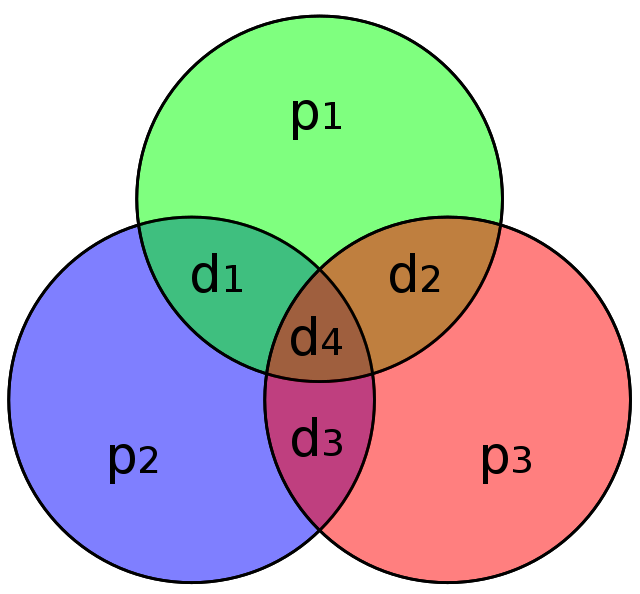
\includegraphics[scale=0.25]{im.png}
		\caption{Результат работы исходного кода}
	\end{figure}
	
	\pagebreak
	Матрица $H$ необходима для восстановление текста и обнаружения ошибки (но только одной!). С её помощью вычисляется так называемый синдром - матрица $S = H\cdot p_1p_2p_3d_1d_2d_3d_4 \text{ (mod 2)}$, показывающая <<сломавшийся>> бит (в этом случае значение синдрома будет совпадать с одним из векторов в матрице $H$).
	
	Как бы ни было удивительно, но мы получаем следующее соотношение между $G$ и $H$: $\text{Im}(G) = \text{Ker}(H)$. Оно выполняется в силу того, что образ $G$ - вектор $p_1p_2p_3d_1d_2d_3d_4$, для которых синдром будет равен 0 (так как никаких вмешательств не было), то есть действие H на $p_1p_2p_3d_1d_2d_3d_4$ даст нам всегда 0. Других же элементов в ядре нет, так как тогда синдром, а значит, и действие H на вектор, не равны 0.
	
	Все вредоносные вмешательства отсекаются поиск синдрома. Если он не равен 0, то мы берём ненулевую строку из него и ищем соответствующей этой строке столбец в $H$, получая номер неисправного бита. Дальше остаётся лишь исправить!
	
	
	\textbf{На этом всё, спасибо!}
	
	
	
\end{document}